\documentclass{article}
\usepackage[utf8]{inputenc}
\usepackage{hyperref}
\usepackage[T1]{fontenc}
\usepackage{lmodern}
\usepackage{cmap}
\usepackage[utf8]{inputenc}
\usepackage[english]{babel}
\usepackage{graphicx}
\usepackage{caption}
\usepackage{subcaption}

\title{Bay Area Bike Share Data Analysis}
\author{Maxim Kovalev\\\texttt{maxim.kovalev@2007.auditory.ru}}
\date{May 2015}


\newcommand{\fix}{\marginpar{FIX}}
\newcommand{\new}{\marginpar{NEW}}


\begin{document}

\maketitle

\begin{abstract}
Here be abstract.
\end{abstract}

\section{...}



\begin{figure}
        \centering
        \begin{subfigure}[b]{0.5\textwidth}
                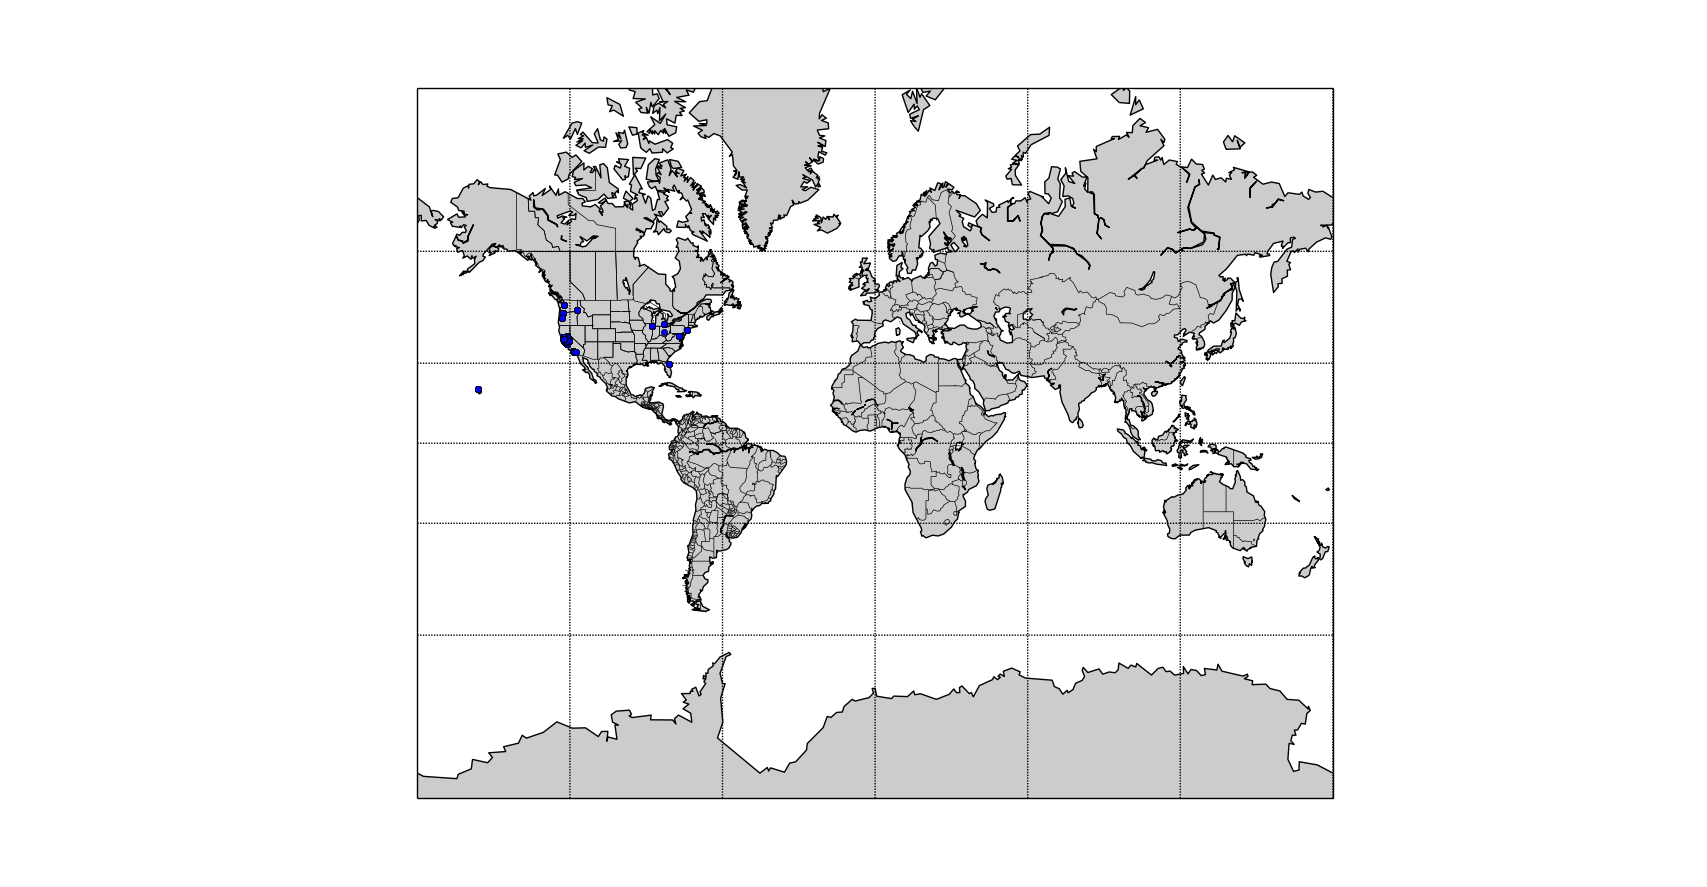
\includegraphics[width=\textwidth]{../home_zips_world.png}
                \caption{On the world map}
                \label{fig:homezips:world}
        \end{subfigure}%
        ~ %add desired spacing between images, e. g. ~, \quad, \qquad, \hfill etc.
          %(or a blank line to force the subfigure onto a new line)
        \begin{subfigure}[b]{0.5\textwidth}
                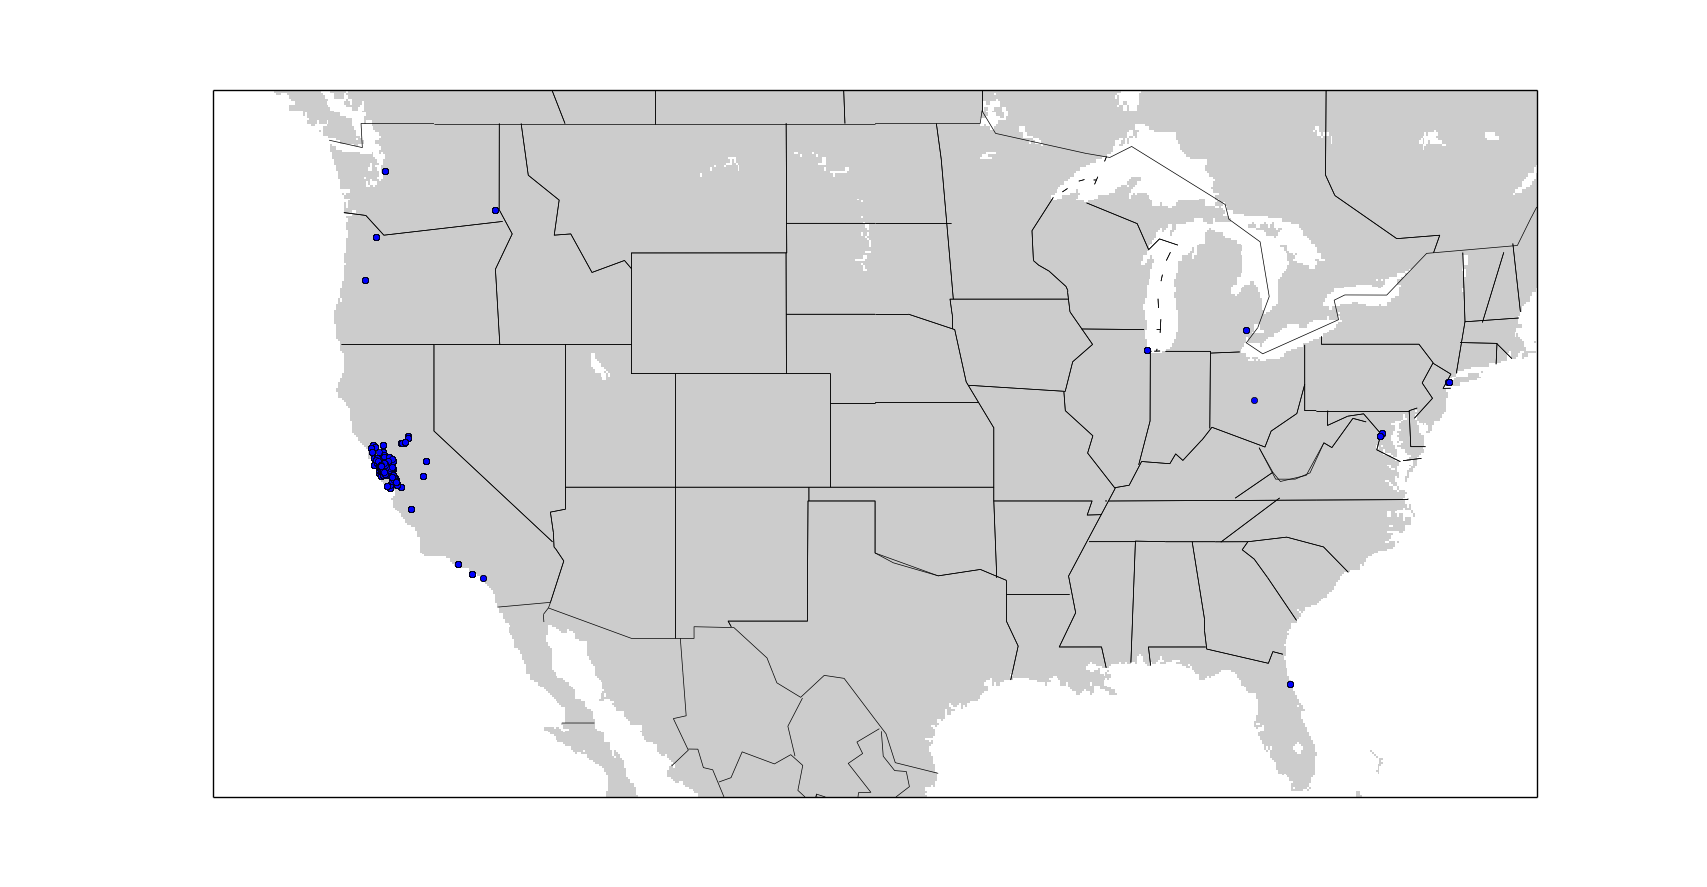
\includegraphics[width=\textwidth]{../home_zips_usa.png}
                \caption{On contiguous states map}
                \label{fig:homezips:usa}
        \end{subfigure}
        ~ %add desired spacing between images, e. g. ~, \quad, \qquad, \hfill etc.
          %(or a blank line to force the subfigure onto a new line)
        \begin{subfigure}[b]{0.4\textwidth}
                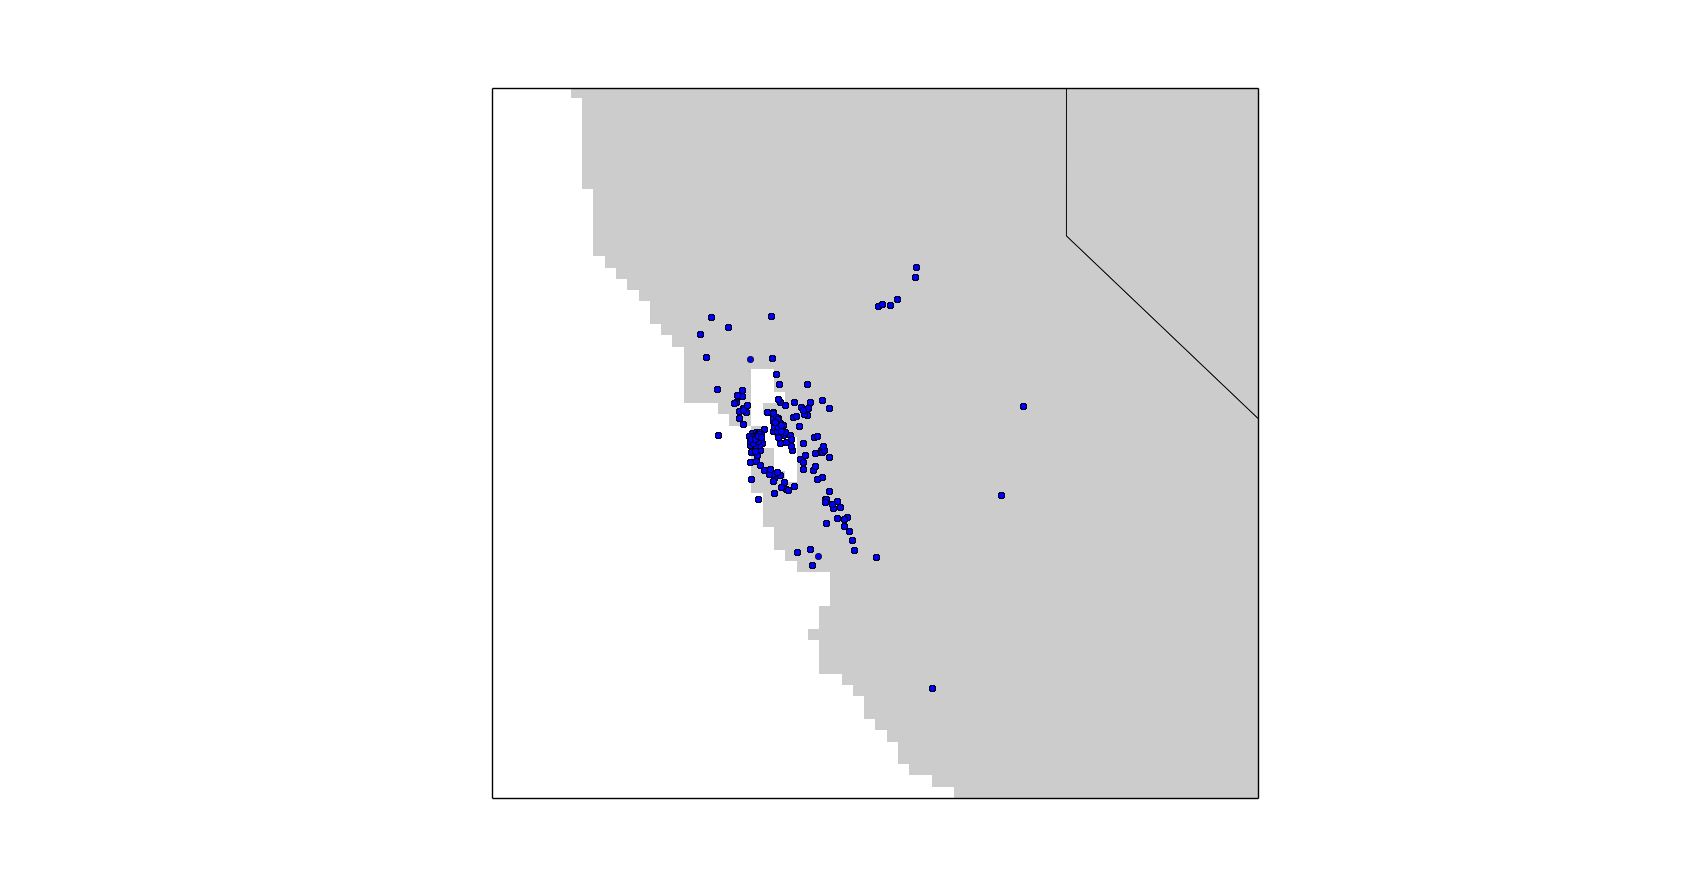
\includegraphics[width=\textwidth]{../home_zips_norcal.png}
                \caption{On Northern California map}
                \label{fig:homezips:norcal}
        \end{subfigure}
        \begin{subfigure}[b]{0.4\textwidth}
                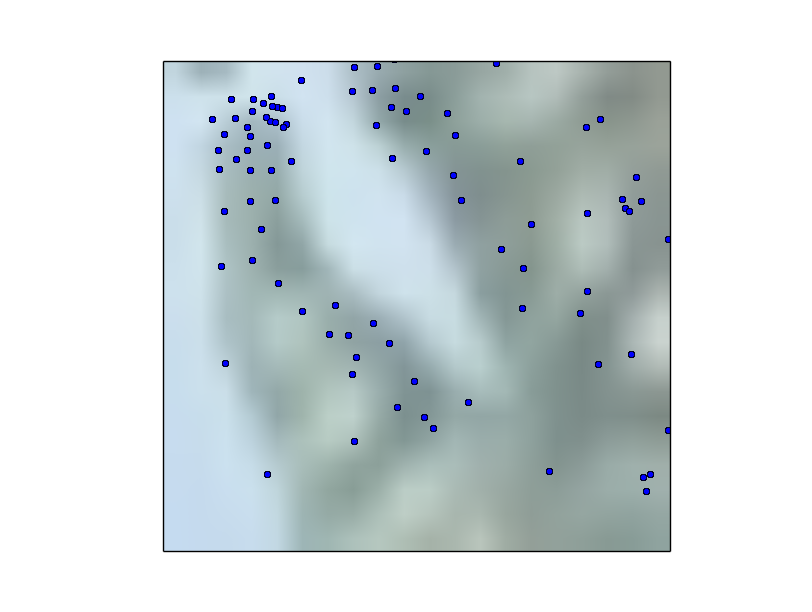
\includegraphics[width=\textwidth]{../home_zips_bay_area.png}
                \caption{On Bay Area map}
                \label{fig:homezips:}
        \end{subfigure}
        \caption{Coordinates of home zip codes of subscribers}
        \label{fig:homezips}
\end{figure}



\end{document}

